
%% bare_jrnl.tex
%% V1.4b
%% 2015/08/26
%% by Michael Shell
%% see http://www.michaelshell.org/
%% for current contact information.
%%
%% This is a skeleton file demonstrating the use of IEEEtran.cls
%% (requires IEEEtran.cls version 1.8b or later) with an IEEE
%% journal paper.
%%
%% Support sites:
%% http://www.michaelshell.org/tex/ieeetran/
%% http://www.ctan.org/pkg/ieeetran
%% and
%% http://www.ieee.org/

%%*************************************************************************
%% Legal Notice:
%% This code is offered as-is without any warranty either expressed or
%% implied; without even the implied warranty of MERCHANTABILITY or
%% FITNESS FOR A PARTICULAR PURPOSE!
%% User assumes all risk.
%% In no event shall the IEEE or any contributor to this code be liable for
%% any damages or losses, including, but not limited to, incidental,
%% consequential, or any other damages, resulting from the use or misuse
%% of any information contained here.
%%
%% All comments are the opinions of their respective authors and are not
%% necessarily endorsed by the IEEE.
%%
%% This work is distributed under the LaTeX Project Public License (LPPL)
%% ( http://www.latex-project.org/ ) version 1.3, and may be freely used,
%% distributed and modified. A copy of the LPPL, version 1.3, is included
%% in the base LaTeX documentation of all distributions of LaTeX released
%% 2003/12/01 or later.
%% Retain all contribution notices and credits.
%% ** Modified files should be clearly indicated as such, including  **
%% ** renaming them and changing author support contact information. **
%%*************************************************************************


% *** Authors should verify (and, if needed, correct) their LaTeX system  ***
% *** with the testflow diagnostic prior to trusting their LaTeX platform ***
% *** with production work. The IEEE's font choices and paper sizes can   ***
% *** trigger bugs that do not appear when using other class files.       ***                          ***
% The testflow support page is at:
% http://www.michaelshell.org/tex/testflow/


%
% If IEEEtran.cls has not been installed into the LaTeX system files,
% manually specify the path to it like:
% \documentclass[journal]{../sty/IEEEtran}
\documentclass[journal]{IEEEtran}

\usepackage{techrep}
\usepackage{indentfirst}
\usepackage{graphicx}
\usepackage{subfigure}
\usepackage{enumerate}
\usepackage{subfigure}

% \setlength{\columnsep}{10mm}
% \setlength{\textwidth}{180mm}
% \setlength{\textheight}{250mm}
% \addtolength{\oddsidemargin}{-9mm}
% \addtolength{\topmargin}{-25mm}

\graphicspath{{figures/}}



% Some very useful LaTeX packages include:
% (uncomment the ones you want to load)


% *** MISC UTILITY PACKAGES ***
%
%\usepackage{ifpdf}
% Heiko Oberdiek's ifpdf.sty is very useful if you need conditional
% compilation based on whether the output is pdf or dvi.
% usage:
% \ifpdf
%   % pdf code
% \else
%   % dvi code
% \fi
% The latest version of ifpdf.sty can be obtained from:
% http://www.ctan.org/pkg/ifpdf
% Also, note that IEEEtran.cls V1.7 and later provides a builtin
% \ifCLASSINFOpdf conditional that works the same way.
% When switching from latex to pdflatex and vice-versa, the compiler may
% have to be run twice to clear warning/error messages.

% *** CITATION PACKAGES ***
%
%\usepackage{cite}
% cite.sty was written by Donald Arseneau
% V1.6 and later of IEEEtran pre-defines the format of the cite.sty package
% \cite{} output to follow that of the IEEE. Loading the cite package will
% result in citation numbers being automatically sorted and properly
% "compressed/ranged". e.g., [1], [9], [2], [7], [5], [6] without using
% cite.sty will become [1], [2], [5]--[7], [9] using cite.sty. cite.sty's
% \cite will automatically add leading space, if needed. Use cite.sty's
% noadjust option (cite.sty V3.8 and later) if you want to turn this off
% such as if a citation ever needs to be enclosed in parenthesis.
% cite.sty is already installed on most LaTeX systems. Be sure and use
% version 5.0 (2009-03-20) and later if using hype rref.sty.
% The latest version can be obtained at:
% http://www.ctan.org/pkg/cite
% The documentation is contained in the cite.sty file itself.

% *** GRAPHICS RELATED PACKAGES ***
%
\ifCLASSINFOpdf{}
  % \usepackage[pdftex]{graphicx}
  % declare the path(s) where your graphic files are
  % \graphicspath{{../pdf/}{../jpeg/}}
  % and their extensions so you won't have to specify these with
  % every instance of \includegraphics
  % \DeclareGraphicsExtensions{.pdf,.jpeg,.png}
\else
  % or other class option (dvipsone, dvipdf, if not using dvips). graphicx
  % will default to the driver specified in the system graphics.cfg if no
  % driver is specified.
  % \usepackage[dvips]{graphicx}
  % declare the path(s) where your graphic files are
  % \graphicspath{{../eps/}}
  % and their extensions so you won't have to specify these with
  % every instance of \includegraphics
  % \DeclareGraphicsExtensions{.eps}
\fi
% graphicx was written by David Carlisle and Sebastian Rahtz. It is
% required if you want graphics, photos, etc. graphicx.sty is already
% installed on most LaTeX systems. The latest version and documentation
% can be obtained at:
% http://www.ctan.org/pkg/graphicx
% Another good source of documentation is "Using Imported Graphics in
% LaTeX2e" by Keith Reckdahl which can be found at:
% http://www.ctan.org/pkg/epslatex
%
% latex, and pdflatex in dvi mode, support graphics in encapsulated
% postscript (.eps) format. pdflatex in pdf mode supports graphics
% in .pdf, .jpeg, .png and .mps (metapost) formats. Users should ensure
% that all non-photo figures use a vector format (.eps, .pdf, .mps) and
% not a bitmapped formats (.jpeg, .png). The IEEE frowns on bitmapped formats
% which can result in "jaggedy"/blurry rendering of lines and letters as
% well as large increases in file sizes.
%
% You can find documentation about the pdfTeX application at:
% http://www.tug.org/applications/pdftex

% *** MATH PACKAGES ***
%
%\usepackage{amsmath}
% A popular package from the American Mathematical Society that provides
% many useful and powerful commands for dealing with mathematics.
%
% Note that the amsmath package sets \interdisplaylinepenalty to 10000
% thus preventing page breaks from occurring within multiline equations. Use:
%\interdisplaylinepenalty=2500
% after loading amsmath to restore such page breaks as IEEEtran.cls normally
% does. amsmath.sty is already installed on most LaTeX systems. The latest
% version and documentation can be obtained at:
% http://www.ctan.org/pkg/amsmath

% *** SPECIALIZED LIST PACKAGES ***
%
%\usepackage{algorithmic}
% algorithmic.sty was written by Peter Williams and Rogerio Brito.
% This package provides an algorithmic environment fo describing algorithms.
% You can use the algorithmic environment in-text or within a figure
% environment to provide for a floating algorithm. Do NOT use the algorithm
% floating environment provided by algorithm.sty (by the same authors) or
% algorithm2e.sty (by Christophe Fiorio) as the IEEE does not use dedicated
% algorithm float types and packages that provide these will not provide
% correct IEEE style captions. The latest version and documentation of
% algorithmic.sty can be obtained at:
% http://www.ctan.org/pkg/algorithms
% Also of interest may be the (relatively newer and more customizable)
% algorithmicx.sty package by Szasz Janos:
% http://www.ctan.org/pkg/algorithmicx

% *** ALIGNMENT PACKAGES ***
%
%\usepackage{array}
% Frank Mittelbach's and David Carlisle's array.sty patches and improves
% the standard LaTeX2e array and tabular environments to provide better
% appearance and additional user controls. As the default LaTeX2e table
% generation code is lacking to the point of almost being broken with
% respect to the quality of the end results, all users are strongly
% advised to use an enhanced (at the very least that provided by array.sty)
% set of table tools. array.sty is already installed on most systems. The
% latest version and documentation can be obtained at:
% http://www.ctan.org/pkg/array

% IEEEtran contains the IEEEeqnarray family of commands that can be used to
% generate multiline equations as well as matrices, tables, etc., of high
% quality.

% *** SUBFIGURE PACKAGES ***
%\ifCLASSOPTIONcompsoc
%  \usepackage[caption=false,font=normalsize,labelfont=sf,textfont=sf]{subfig}
%\else
%  \usepackage[caption=false,font=footnotesize]{subfig}
%\fi
% subfig.sty, written by Steven Douglas Cochran, is the modern replacement
% for subfigure.sty, the latter of which is no longer maintained and is
% incompatible with some LaTeX packages including fixltx2e. However,
% subfig.sty requires and automatically loads Axel Sommerfeldt's caption.sty
% which will override IEEEtran.cls' handling of captions and this will result
% in non-IEEE style figure/table captions. To prevent this problem, be sure
% and invoke subfig.sty's "caption=false" package option (available since
% subfig.sty version 1.3, 2005/06/28) as this is will preserve IEEEtran.cls
% handling of captions.
% Note that the Computer Society format requires a larger sans serif font
% than the serif footnote size font used in traditional IEEE formatting
% and thus the need to invoke different subfig.sty package options depending
% on whether compsoc mode has been enabled.
%
% The latest version and documentation of subfig.sty can be obtained at:
% http://www.ctan.org/pkg/subfig

% *** FLOAT PACKAGES ***
%
%\usepackage{fixltx2e}
% fixltx2e, the successor to the earlier fix2col.sty, was written by
% Frank Mittelbach and David Carlisle. This package corrects a few problems
% in the LaTeX2e kernel, the most notable of which is that in current
% LaTeX2e releases, the ordering of single and double column floats is not
% guaranteed to be preserved. Thus, an unpatched LaTeX2e can allow a
% single column figure to be placed prior to an earlier double column
% figure.
% Be aware that LaTeX2e kernels dated 2015 and later have fixltx2e.sty's
% corrections already built into the system in which case a warning will
% be issued if an attempt is made to load fixltx2e.sty as it is no longer
% needed.
% The latest version and documentation can be found at:
% http://www.ctan.org/pkg/fixltx2e

%\usepackage{stfloats}
% stfloats.sty was written by Sigitas Tolusis. This package gives LaTeX2e
% the ability to do double column floats at the bottom of the page as well
% as the top. (e.g., "\begin{figure*}[!b]" is not normally possible in
% LaTeX2e). It also provides a command:
%\fnbelowfloat
% to enable the placement of footnotes below bottom floats (the standard
% LaTeX2e kernel puts them above bottom floats). This is an invasive package
% which rewrites many portions of the LaTeX2e float routines. It may not work
% with other packages that modify the LaTeX2e float routines. The latest
% version and documentation can be obtained at:
% http://www.ctan.org/pkg/stfloats
% Do not use the stfloats baselinefloat ability as the IEEE does not allow
% \baselineskip to stretch. Authors submitting work to the IEEE should note
% that the IEEE rarely uses double column equations and that authors should try
% to avoid such use. Do not be tempted to use the cuted.sty or midfloat.sty
% packages (also by Sigitas Tolusis) as the IEEE does not format its papers in
% such ways.
% Do not attempt to use stfloats with fixltx2e as they are incompatible.
% Instead, use Morten Hogholm'a dblfloatfix which combines the features
% of both fixltx2e and stfloats:
%
% \usepackage{dblfloatfix}
% The latest version can be found at:
% http://www.ctan.org/pkg/dblfloatfix

%\ifCLASSOPTIONcaptionsoff
%  \usepackage[nomarkers]{endfloat}
% \let\MYoriglatexcaption\caption
% \renewcommand{\caption}[2][\relax]{\MYoriglatexcaption[#2]{#2}}
%\fi
% endfloat.sty was written by James Darrell McCauley, Jeff Goldberg and
% Axel Sommerfeldt. This package may be useful when used in conjunction with
% IEEEtran.cls'  captionsoff option. Some IEEE journals/societies require that
% submissions have lists of figures/tables at the end of the paper and that
% figures/tables without any captions are placed on a page by themselves at
% the end of the document. If needed, the draftcls IEEEtran class option or
% \CLASSINPUTbaselinestretch interface can be used to increase the line
% spacing as well. Be sure and use the nomarkers option of endfloat to
% prevent endfloat from "marking" where the figures would have been placed
% in the text. The two hack lines of code above are a slight modification of
% that suggested by in the endfloat docs (section 8.4.1) to ensure that
% the full captions always appear in the list of figures/tables - even if
% the user used the short optional argument of \caption[]{}.
% IEEE papers do not typically make use of \caption[]'s optional argument,
% so this should not be an issue. A similar trick can be used to disable
% captions of packages such as subfig.sty that lack options to turn off
% the subcaptions:
% For subfig.sty:
% \let\MYorigsubfloat\subfloat
% \renewcommand{\subfloat}[2][\relax]{\MYorigsubfloat[]{#2}}
% However, the above trick will not work if both optional arguments of
% the \subfloat command are used. Furthermore, there needs to be a
% description of each subfigure *somewhere* and endfloat does not add
% subfigure captions to its list of figures. Thus, the best approach is to
% avoid the use of subfigure captions (many IEEE journals avoid them anyway)
% and instead  reference/explain all the subfigures within the main caption.
% The latest version of endfloat.sty and its documentation can obtained at:
% http://www.ctan.org/pkg/endfloat
%
% The IEEEtran \ifCLASSOPTIONcaptionsoff conditional can also be used
% later in the document, say, to conditionally put the References on a
% page by themselves.

% *** PDF, URL AND HYPERLINK PACKAGES ***
%
%\usepackage{url}
% url.sty was written by Donald Arseneau. It provides better support for
% handling and breaking URLs. url.sty is already installed on most LaTeX
% systems. The latest version and documentation can be obtained at:
% http://www.ctan.org/pkg/url
% Basically, \url{my_url_here}.

% *** Do not adjust lengths that control margins, column widths, etc. ***
% *** Do not use packages that alter fonts (such as pslatex).         ***
% There should be no need to do such things with IEEEtran.cls V1.6 and later.
% (Unless specifically asked to do so by the journal or conference you plan
% to submit to, of course. )


% correct bad hyphenation here
\hyphenation{op-tical net-works semi-conduc-tor}


\begin{document}
%
% paper title
% Titles are generally capitalized except for words such as a, an, and, as,
% at, but, by, for, in, nor, of, on, or, the, to and up, which are usually
% not capitalized unless they are the first or last word of the title.
% Linebreaks \\ can be used within to get better formatting as desired.
% Do not put math or special symbols in the title.

% title
% \title{Bare Demo of IEEEtran.cls\\ for IEEE Journals}

%
%
% author names and IEEE memberships
% note positions of commas and nonbreaking spaces ( ~ ) LaTeX will not break
% a structure at a ~ so this keeps an author's name from being broken across
% two lines.
% use \thanks{} to gain access to the first footnote area
% a separate \thanks must be used for each paragraph as LaTeX2e's \thanks
% was not built to handle multiple paragraphs
%

% auther
% \author{Michael~Shell,~\IEEEmembership{Member,~IEEE,}
%         John~Doe,~\IEEEmembership{Fellow,~OSA,}
%         and~Jane~Doe,~\IEEEmembership{Life~Fellow,~IEEE}% <-this % stops a space
% \thanks{M. Shell was with the Department
% of Electrical and Computer Engineering, Georgia Institute of Technology, Atlanta,
% GA, 30332 USA e-mail: (see http://www.michaelshell.org/contact.html).}% <-this % stops a space
% \thanks{J. Doe and J. Doe are with Anonymous University.}% <-this % stops a space
% \thanks{Manuscript received April 19, 2005; revised August 26, 2015.}}


% note the % following the last \IEEEmembership and also \thanks -
% these prevent an unwanted space from occurring between the last author name
% and the end of the author line. i.e., if you had this:
%
% \author{....lastname \thanks{...} \thanks{...} }
%                     ^------------^------------^----Do not want these spaces!
%
% a space would be appended to the last name and could cause every name on that
% line to be shifted left slightly. This is one of those "LaTeX things". For
% instance, "\textbf{A} \textbf{B}" will typeset as "A B" not "AB". To get
% "AB" then you have to do: "\textbf{A}\textbf{B}"
% \thanks is no different in this regard, so shield the last } of each \thanks
% that ends a line with a % and do not let a space in before the next \thanks.
% Spaces after \IEEEmembership other than the last one are OK (and needed) as
% you are supposed to have spaces between the names. For what it is worth,
% this is a minor point as most people would not even notice if the said evil
% space somehow managed to creep in.



% The paper headers
% \markboth{Journal of \LaTeX\ Class Files,~Vol.~14, No.~8, August~2015}%
% {Shell \MakeLowercase{\textit{et al.}}: Bare Demo of IEEEtran.cls for IEEE Journals}

% The only time the second header will appear is for the odd numbered pages
% after the title page when using the twoside option.
%
% *** Note that you probably will NOT want to include the author's ***
% *** name in the headers of peer review papers.                   ***
% You can use \ifCLASSOPTIONpeerreview for conditional compilation here if
% you desire.




% If you want to put a publisher's ID mark on the page you can do it like
% this:
%\IEEEpubid{0000--0000/00\$00.00~\copyright~2015 IEEE}
% Remember, if you use this you must call \IEEEpubidadjcol in the second
% column for its text to clear the IEEEpubid mark.



% use for special paper notices
%\IEEEspecialpapernotice{(Invited Paper)}




% make the title area
% \maketitle

% As a general rule, do not put math, special symbols or citations
% in the abstract or keywords.
% \begin{abstract}
% The abstract goes here.
% \end{abstract}

% Note that keywords are not normally used for peerreview papers.
% \begin{IEEEkeywords}
% IEEE, IEEEtran, journal, \LaTeX, paper, template.
% \end{IEEEkeywords}


% For peer review papers, you can put extra information on the cover
% page as needed:
% \ifCLASSOPTIONpeerreview
% \begin{center} \bfseries EDICS Category: 3-BBND \end{center}
% \fi
%
% For peerreview papers, this IEEEtran command inserts a page break and
% creates the second title. It will be ignored for other modes.
\IEEEpeerreviewmaketitle{}
% Introduction
% First paragraph of paper need be big Alhabet
\section{Introduction}
\IEEEPARstart{T}{his} document is a template for Microsoft Word versions 6.0 or later. If you are reading a paper or PDF version of this doconference. (By Eric)

\section{Related Work}
(By Eric)

% An example of a floating figure using the graphicx package.
% Note that \label must occur AFTER (or within) \caption.
% For figures, \caption should occur after the \includegraphics.
% Note that IEEEtran v1.7 and later has special internal code that
% is designed to preserve the operation of \label within \caption
% even when the captionsoff option is in effect. However, because
% of issues like this, it may be the safest practice to put all your
% \label just after \caption rather than within \caption{}.
%
% Reminder: the "draftcls" or "draftclsnofoot", not "draft", class
% option should be used if it is desired that the figures are to be
% displayed while in draft mode.
%
%\begin{figure}[!t]
%\centering
%\includegraphics[width=2.5in]{myfigure}
% where an .eps filename suffix will be assumed under latex,
% and a .pdf suffix will be assumed for pdflatex; or what has been declared
% via \DeclareGraphicsExtensions.
%\caption{Simulation results for the network.}
%\label{fig_sim}
%\end{figure}

% Note that the IEEE typically puts floats only at the top, even when this
% results in a large percentage of a column being occupied by floats.


% An example of a double column floating figure using two subfigures.
% (The subfig.sty package must be loaded for this to work.)
% The subfigure \label commands are set within each subfloat command,
% and the \label for the overall figure must come after \caption.
% \hfil is used as a separator to get equal spacing.
% Watch out that the combined width of all the subfigures on a
% line do not exceed the text width or a line break will occur.
%
%\begin{figure*}[!t]
%\centering
%\subfloat[Case I]{\includegraphics[width=2.5in]{box}%
%\label{fig_first_case}}
%\hfil
%\subfloat[Case II]{\includegraphics[width=2.5in]{box}%
%\label{fig_second_case}}
%\caption{Simulation results for the network.}
%\label{fig_sim}
%\end{figure*}
%
% Note that often IEEE papers with subfigures do not employ subfigure
% captions (using the optional argument to \subfloat[]), but instead will
%  reference/describe all of them (a), (b), etc., within the main caption.
% Be aware that for subfig.sty to generate the (a), (b), etc., subfigure
% labels, the optional argument to \subfloat must be present. If a
% subcaption is not desired, just leave its contents blank,
% e.g., \subfloat[].


% An example of a floating table. Note that, for IEEE style tables, the
% \caption command should come BEFORE the table and, given that table
% captions serve much like titles, are usually capitalized except for words
% such as a, an, and, as, at, but, by, for, in, nor, of, on, or, the, to
% and up, which are usually not capitalized unless they are the first or
% last word of the caption. Table text will default to \footnotesize as
% the IEEE normally uses this smaller font for tables.
% The \label must come after \caption as always.
%
%\begin{table}[!t]
%% increase table row spacing, adjust to taste
%\renewcommand{\arraystretch}{1.3}
% if using array.sty, it might be a good idea to tweak the value of
% \extrarowheight as needed to properly center the text within the cells
%\caption{An Example of a Table}
%\label{table_example}
%\centering
%% Some packages, such as MDW tools, offer better commands for making tables
%% than the plain LaTeX2e tabular which is used here.
%\begin{tabular}{|c||c|}
%\hline
%One & Two\\
%\hline
%Three & Four\\
%\hline
%\end{tabular}
%\end{table}


% Note that the IEEE does not put floats in the very first column
% - or typically anywhere on the first page for that matter. Also,
% in-text middle ("here") positioning is typically not used, but it
% is allowed and encouraged for Computer Society conferences (but
% not Computer Society journals). Most IEEE journals/conferences use
% top floats exclusively.
% Note that, LaTeX2e, unlike IEEE journals/conferences, places
% footnotes above bottom floats. This can be corrected via the
% \fnbelowfloat command of the stfloats package.



\section{vCPE System Overview}
\subsection{Overview of Network Function}\label{ssec:nfv_overview}
With the concept of SDN-enabled\cite{sdn-enabled} VNFs, SDN technology work not only a for traffic steering but also as a part of network functions. In this idea, network function have been achieved by the synergies between compute and network infrastructures. The former is a VNF controller, mainly responsible for dealing with stateful processing. The latter is a SDN switch, used for stateless processing.

\subsubsection{Stateful Processing component (VNF controller in container)}
This component have to control the workflow, keep the state associated with the VNF, and provide interface for service providers or customers to configure and update the behavior of the stateless datapath processing component. We use SDN controller to implement the NFV controller and it’s worth noting that we use southbound APIs of SDN controller framework to handle the interface between the stateful and stateless component with OpenFlow protocol, which was originally designed for this.

\subsubsection{Stateless Processing component (SDN datapath)}
Stateless processing component, are implemented by SDN datapath resources, which is optimized for data plane traffic processing. Since SDN switch have decoupled the control plane and data plane, so it can accept the control message from the stateful processing component.

Using the advantages of this architecture, we can assign stateless or light-weight state work to the SDN switch, for example, packet filtering and packet counting, to load-off the computing resources. If we want to update our service, we just need to update the statful component, since the stateless component just follow the command from stateful components.

\begin{figure}[!t]
\centering
\caption{Overview of network function}
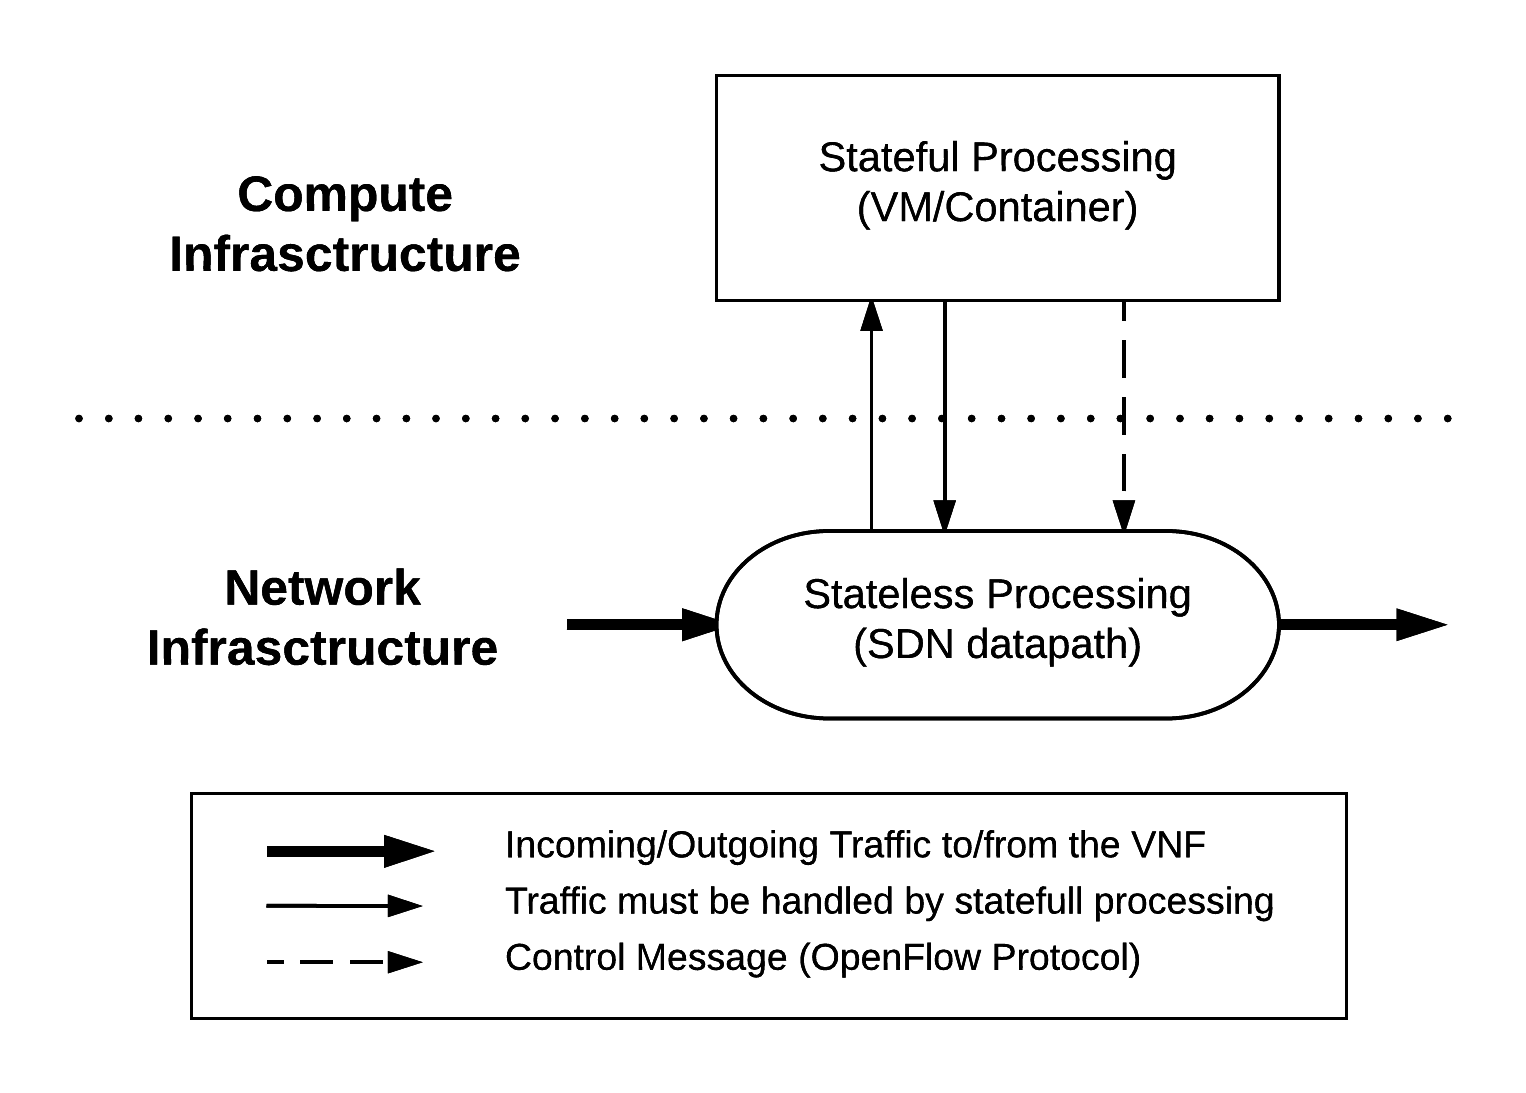
\includegraphics[width=3in]{./figures/nfv_overview}
\label{fig:nfv_overview}
\end{figure}


\subsection{Service Deployment Model}\label{ssec:vcpe_deploy}

\begin{figure}[!t]
\centering
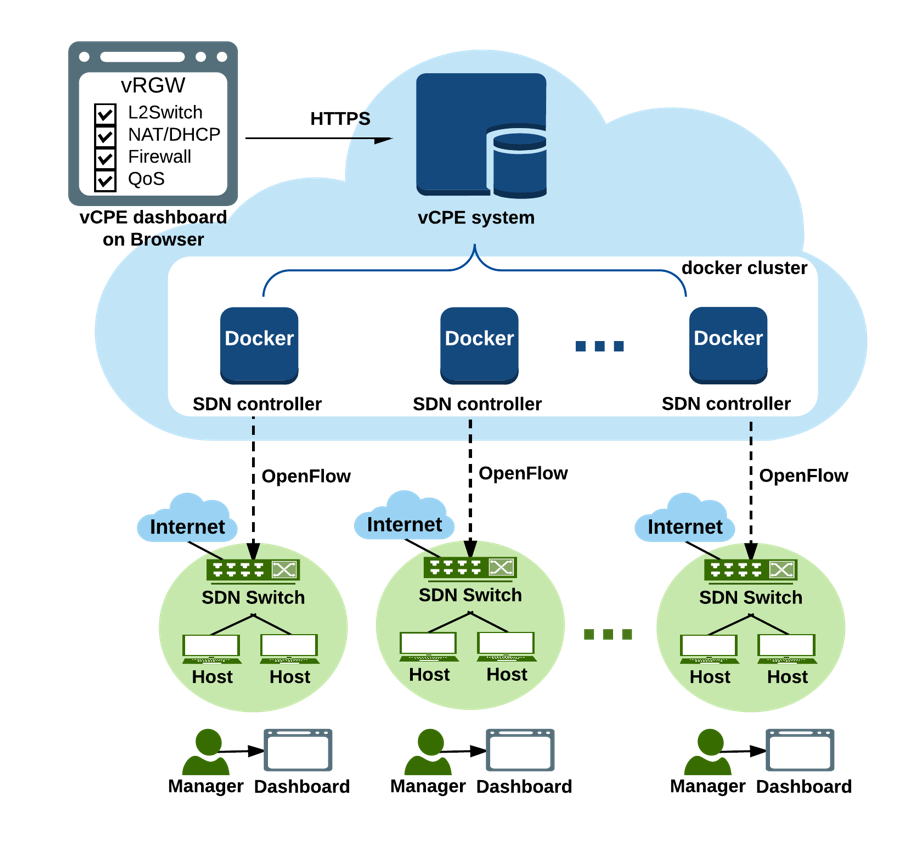
\includegraphics[width=3in]{./figures/deployment}
\caption{Service Deployment Model}
\label{fig:vcpe_deploy}
\end{figure}

With architecture mentioned in \ref{ssec:nfv_overview}, we come up with a network function service deployment model. Because computing infrastructures handles the algorithm and policies, and the generic network devices only do stateless processing, the customer just need to buy a general SDN switch at their home gateway and will have a different network function service by subscribing different NFV controller through our vCPE platform.

Figure \ref{fig:vcpe_deploy} illustrates the service deployment model. Each green area is a local network domain of customer. At the gateway of this domain, there’s a SDN-enabled switch. The customer can subscribe to our vCPE service through our dashboard. After subscribing, the vCPE system will create a new docker container, in which running a SDN controller we developed. The customer only need to setup the gateway SDN switch to connect the SDN controller by the OpenFlow protocol, then the switch will handle these service.

\subsection{Architecture of the vCPE framework}
\subsubsection{System Overview}

\begin{figure}[!t]
\centering
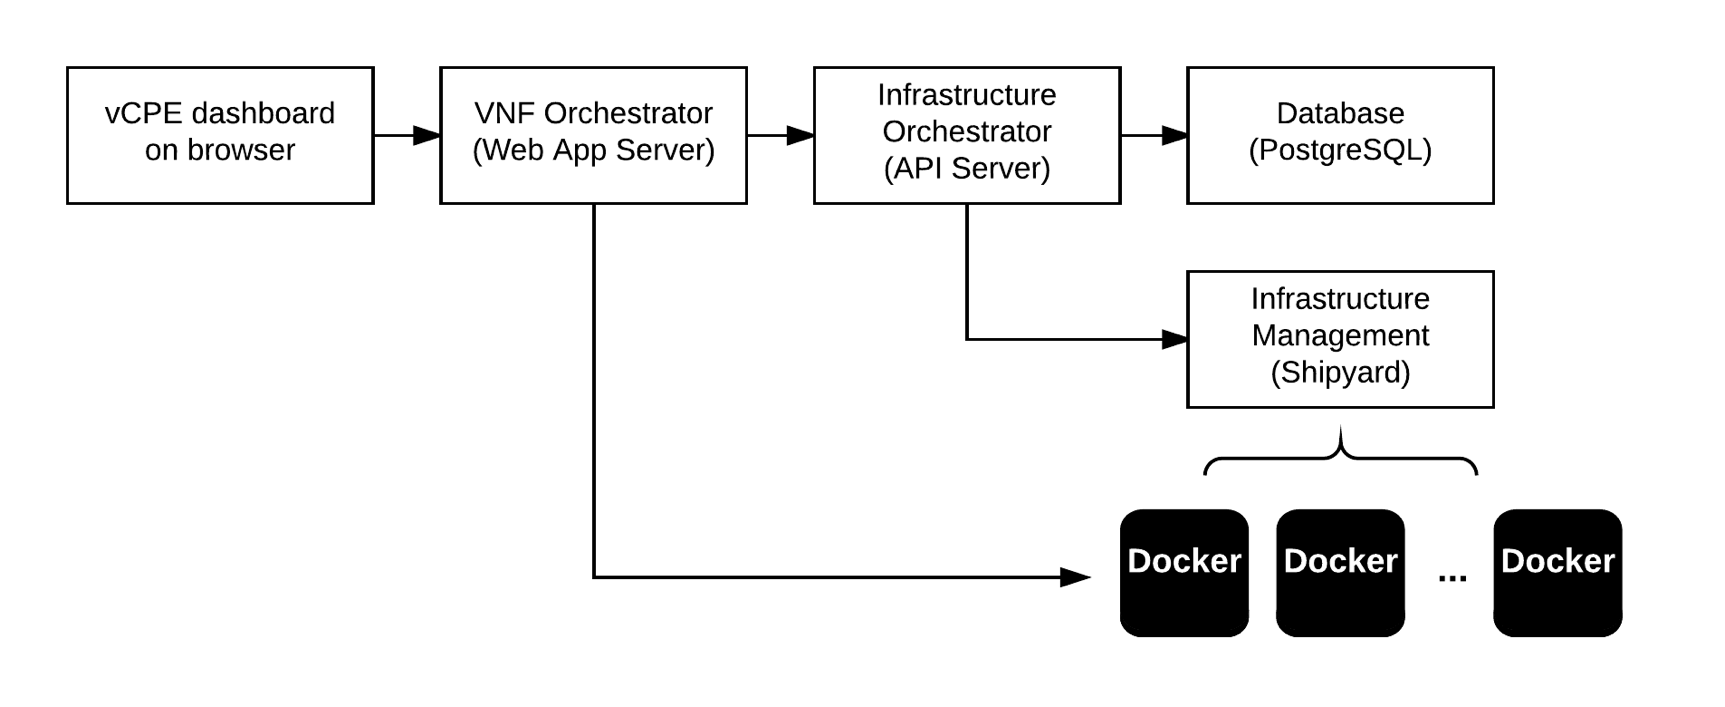
\includegraphics[width=3in]{./figures/vcpe_framework_overview}
\caption{Overview of vCPE framework}
\label{fig:vcpe_framework}
\end{figure}

The architecture as shown in Fig \ref{fig:vcpe_framework} including of a Infrastructure Controller,
% Fig lable to change
Infrastructure Orchestrator, Cloud Database, VNF Controllers and VNF Orchestrator.
The Infrastructure Orchestrator, VNF Orchestrator and Cloud Database are web servers
Each component is introduced in the subsection below.

\subsubsection{Infrastructure Controller}
The infrastructure controller is a composed Docker management server
with the ability to manage the Docker resources like containers and images.
The infrastructure doesn't handle the customer authentication or maintaining the state of running service,
it just follows the request from the infrastructure orchestrator to create, delete, start, stop and inspect containers.

\subsubsection{Infrastructure Orchestrator}
The infrastructure orchestrator plays the key role of our system.
It connecting and automating of workflows when we deploy our services.
When a customer subscribes, the infrastructure orchestrator authenticates the customer first,
next it will call the infrastructure controller to create a container for this customer,
and update information in database afterwards. It handle the entire lifecycle of our vCPE service.

\subsubsection{Cloud Database}
The cloud database is used for restoring the of our vCPE services,
which include each customer’s credential, customer’s container settings and virtual CPE service states.
The cloud database is using PostgreSQL, which is a open source, easily customized and object-relational database system.
Only Infrastructure Orchestrator has permissions to access cloud database.

\subsubsection{VNF Controllers}
VNF Controllers contains a SDN controller developed with ryu framework and a remote launcher module.
The SDN controller does not have a remote launcher module to remotely execute a SDN controller.
We built a light-weight server as a launcher module to resolve the remotely execution issue.
The remote launcher module monitor the SDN controller process ID (PID)
and properly kill the SDN controller process ID when on demand.
When the infrastructure controller once create the container, the remote module will run up initially, waiting request  from VNF Orchestrator. The details of SDN controller design will be presented at section \ref{sec:nf_mft}.

\subsubsection{VNF Orchestrator}
The VNF Orchestrator is a Web application server hosting on Amazon Web server,
being online for customer and provide a dashboard for virtual CPE and containers management and configuration.

Through the web UI provided by the VNF Orchestrator,
the customers can subscribe to the desired service and without typing any command via the command line interface (CLI).
After receiving the subscribing message, the VNF orchestrator will request the infrastructure orchestrator to create a new VNF controller,
and then send the virtual CPE configuration to the new VNF controller.
Based on configuration demands under different conditions,
the network administrator is able to select any of the listed network functions on the dashboard
such as Firewall, NAT, DHCP and QoS management.


\subsection{Network Functions}
\subsubsection{Firewall}
The firewall service could filter the packets based on packet header fields, including MAC address, IP, and layer4 protocols.
The network manager can add new rules or remove rules to the access control list through our vCPE GUI.

\subsubsection{NAT}
The NAT service is a network function that can remap  IP address to another one.
The Source NAT (SNAT) is typically used by internal users (inside private network) to access the Internet (outside network).
The network function uses the action “Set-Field”, which defined by OpenFlow protocol for rewriting packet header fields.
Via vCPE GUI interface, the network manager can set up the WAN port of SDN switch,
public IP, default gateway, and local network address when using this function.

\subsubsection{DHCP}
DHCP service allocates IP addresses to hosts dynamically. To implement the function, the SDN controller cope with UDP packets which use port 67 and 68. It generates DHCP offer and DHCP acknowledge to reply DHCP discovery and DHCP request received from the hosts.

\subsubsection{Forwarding}
Forwarding Service is a basic service that forward traffic to its destination
and we use the Mac address learning concept to implement our forwarding function.

\subsubsection{QoS}
Quality of Service (QoS) are always used to control the traffic flows of a network
and prevent the traffic to exceed the network capacity and cause traffic congestion.
Therefore we implement the bandwidth management using meter
which is defined within OpenFlow protocol 1.3 to set the limitation of the bandwidth.
Beside achieving network functions virtualization with SDN technology,
we also make the network administrator manage and monitor a network more easily.
As a result, we can offer the user the best network quality in the limited network resource without traffic congestion.
In this paper, our QoS integrates with a flow classification engine
and offers the three ways of bandwidth management:
\begin{itemize}
\item For a specific host..
\item For a specific host.
\item For a specific application from a host or a domain.
\end{itemize}


\subsection{Application Identification}
Application identification is to identify each flow
as an application name to enable QoS management system to do bandwidth control or distribution at application level.
A flow is defined by 5-tuple (source IP, source port, destination IP, destination port, and transport layer protocol).
Applications include desktop applications, native mobile applications, and web applications,
such as Facebook, Skype, YouTube, Instagram, Line and WeChat.
We use supervised machine learning and a method based on inspecting domain name service (DNS) responses to do flow classification.
After application identification system classifies a flow as an application name,
it sends the classification result to a server with database.
The server stores the classification result into database, and waits for query with 5-tuple from QoS management system.
The detail will be described in section \ref{sec:app_classification}.



\section{Network function with multiple table management model}\label{sec:nf_mft}
\subsection{Multiple Flow Tables Strategy}
In subsection \ref{ssec:nfv_overview}, the vCPE service design architecture have been introduced. The network functions are handled by the cooperation between SDN controller on cloud and SDN switch at the local network gateway. The controller transform the network functions to series of OpenFlow rules requests and send to SDN switch. Following the orders from controller, the SDN switch inserts rules to its flow tables, checks incoming packets against the flow entry match fields, and execute the actions in matching rules. The flow table defines all matching and corresponding processing, thus playing an important role to executive network function.

Since the flow table is crucial component, and we find that single table binds us to implement our network functions. The \cite{onf-multi-tables} also mentioned two condition for single table is too restrictive. The first is a single packet need to perform independent actions based on matching different fields. The second is that the packet needs two-stage processing. Involves into both situation, our network functions implemented by multiple flow tables strategy.

In multiple flow tables strategy, the most important question is: which flow table should we insert rules into? We use the network function as a demarcation, that is, SDN applications which are responsible for specific network functions will only insert rules to one specific flow table, so we can focus on the design of the network function itself. In this way, however, the order of flow table become crucial. Should we put this network function at first, or the other? The answer is about the type of match and action in the rules generated by the network function

The network functions of our vCPE services including Forwarding, Firewall, NAT, DHCP and QoS. We have determined the order of each function, shown in \ref{fig:table-seq}.  In the following subsections, we will introduce how to implement these network functions, which type of rules will be inserted to SDN switch, and how these rules affect our decision of the order of flow tables.

\begin{figure}[!t]
\centering
\includegraphics[width=3in]{./figures/multiple_table}
\caption{The flow table order of our vCPE service}
\label{fig:table-seq}
\end{figure}


\subsection{Service Control}
Service control is used to enable or disable service. To enable a service, we need to modify the table-miss rule. We always put a packet-in rule in the table of the last active service as a table-miss in case that there isn't any corresponding rule. To make our service chain possible, the rules of each service except the last service contains an additional action, go to next table, so the packets can continue to pass through all active services.

To disable a service, we not only need to modify the table-miss rule but also have to add an enforce rule. Each enforce rules has maximum priority and the action is goto next table. It means that packets will still pass through the disabled service's table, and the only thing they do in this table is ignoring other rules and go to next table.


\subsection{Firewall}
Firewall service is able to block traffic dynamically, and in this service, the packets will not cause any packet-in event.
On the dashboard, we can specify the blocking policies. There are 4 kinds of policies:
\begin{itemize}
\item Block any traffic from a certain source IP.
\item Block all traffic to a certain destination IP.
\item Block traffic based on known layer 4 protocols, such as SSH, HTTP, etc.
\item Block traffic to any layer 4 ports of a host.
\end{itemize}

For different policies, the controller applies corresponding rules to the SDN switch. After the policies are set, the blocking rules will be installed immediately. Then any traffic that hit the blocking rules will be dropped. For normal traffic, they will not be affected.

As shown in Table \ref{table:fw}, all the actions of flow entries are drop. The 1st rule illustrates that SSH connection with source IP address 192.168.2.1 would be blocked. The 2nd rule shows the flow entry would block the Telnet protocol.

In our multiple table model, the firewall service is located in the table 1, since once packets are caught by the blocking rules, they doesn't need to apply any other services. The packets which match the rules will be dropped immediately, and their journey in the flow table ends here. To other no-blocked packets, they pass all blocking rules and finally match the table-miss rule, which will let the packets go on the next table. The action of firewall is different from other services, since in other services, no matter what actions are taken to the packets, the packets have to go to the next table

\begin{table*}[]
\centering
\caption{Firewall rules in Flow Entry}
\begin{threeparttable}
\label{table:fw}
\begin{tabular}{|l|l|l|l|l|l|}
\hline
IP proto & IP Src      & IP Dst       & L4 sport & L4 dport & Action \\ \hline
TCP      & 192.168.2.1 & *            & *        & 22       & Drop   \\ \hline
TCP      & *           & *            & *        & 23       & Drop   \\ \hline

\end{tabular}
\begin{tablenotes}
  \small
  \item Symbol * represents wildcard (match any value).
\end{tablenotes}
\end{threeparttable}
\end{table*}


\subsection{DHCP}



\subsection{NAT}
\begin{figure}[!t]
\centering
\includegraphics[width=3in]{./figures/nat_illustrate}
\caption{Illustration of NAT service}
\label{fig:nat_illustration}
\end{figure}
The NAT service could allow a lot of hosts to use one public IP address to connect the network.
In order to achieve this thing, SDN controller have to set the packet header filed.
Because the SDN switch would set the field, the first packet have to go to controller.
And controller would add the flow to SDN switch, after that the packet would not go to controller.
It can decrease the burdens of the controller.

Below is a examples to show how the NAT service modify the IP address and port number,
as shown in Fig \ref{fig:nat_illustration}.

For outgoing packet, SDN switch doesn’t have any flow entry in flow table,
so the Packet-in event will be triggered at the beginning.
The packet that is sent by private network host will be sent to SDN controller,
and the packet header fields are modified by Set-Field action.
The source IP address and source port number of outgoing packet will be modified to public IP address
and remaped a new port number for NAT.
For ingoing packet, the destination IP and destination port number are modified to fit private IP and port number.
And then SDN controller add these flow entries to SDN switch, it can’t avoid that all the packet sent to controller.
Fig. \ref{fig:nat_illustration} show the public IP address of NAT is 140.114.71.178 and a host private IP is 192.168.8.254 and port number 7878. The client sent the packet to a server with IP address 140.114.71.177 and port number 9898.

As shown in Table \ref{table:nat}, when host sent the packet to server (outgoing),
the Packet-in will be trigger, and then packet to controller.
The Set-Field action would modify the Source IP to public IP address of NAT is 140.114.71.178 and source port to 2000.
when the server sends back to the client (ingoing), the packet header field would be modified.
The destination IP address and destination port number would be modified to 192.168.8.254 and 7788.

\begin{table*}[]
\centering
\caption{Flow entry for modifying the packet header fields of packets}
\label{table:nat}
\begin{tabular}{|l|l|l|l|l|l|}
\hline
            &IP Src          & IP Dst          & L4 src port  & L4 dst port & Action                                                                            \\ \hline
1. outgoing &192.168.8.254   &140.114.71.177   & 7878         & 9898        & \begin{tabular}[c]{@{}l@{}}IP Src $\,\to\,$ 140.114.71.178; \\ L4 src port $\,\to\,$ 2000\end{tabular} \\ \hline
2. ingoing  &140.114.71.177  &140.114.71.178   & 9898         & 2000        & \begin{tabular}[c]{@{}l@{}}IP Dst $\,\to\,$ 192.168.8.254; \\ L4 dst port $\,\to\,$ 7878\end{tabular} \\ \hline
\end{tabular}
\end{table*}

In the single table framework, we have to add the two rules to SDN switch to match the outgoing and ingoing situation.
At the first, we predict the NAT service to be put one the last table in the multiple table framework.
Because the NAT service need to set the packet header fields and play a role of connection to the outside network.
And the most important thing is that the SDN switch is according to order of table to match.
We have to consider the outgoing and ingoing situations.
As a result of all the above factors combined,
the NAT service is located at the first and the last table in our multiple table framework.


\subsection{QoS}
\subsection{Forwarding}
In this service, when the first packet in a new connection incoming, it will cause a packet-in event because there is no corresponding rule. When controller receives the packet, it will record IP-layer information, including source IP, destination IP, input port number, source mac address and destination mac address. With the recorded information, the controller is able to install a 5-tuple forwarding rule for this connection and following packets don’t need to packet-in again. The 5-tuple is source IP, destination IP, network layer protocol, source layer 4 port, and destination layer 4 port.

In order to gather per-session statistics information, 5-tuple rules are needed. This is why we don’t add rules  based on mac address.  The controller installs a pair of dummy rules for every connection, and then request the switch to get current flow statistics every second. In this way, we can get the real-time bandwidth statistics of each connection by just subtracting the byte count from byte count of last second.



\section{Application Identifier method} \label{sec:app_classification}
In order to let QoS management system be able to control or distribute bandwidth at application level, we designed and implemented an application identification system (also called flow classification system) to judge each flow is established by what application. In other words, the system can classify each flow as an application name in real time, rather than a rough category or a transport layer protocol.
We use supervised machine learning (ML) and a method based on inspecting domain name service (DNS) responses to do flow classification. Except for DNS responses, the system only analyzes transport layer information of packets without inspecting their payload


\subsection{Architecture of our application identification system}
There are training phase (also called preparation phase) and classifying phase, their architectures are shown in Fig \ref{fig:classifcation_training} and Fig \ref{fig:classifcation_classifying} respectively. These architectures can be integrated, and do training and classifying in the same time. The detail will be mentioned in the following paragraph

\begin{figure}[!t]
\centering
\includegraphics[width=3in]{./figures/classification_training}
\caption{Architecture of our application identification system in training phase}
\label{fig:classifcation_training}
\end{figure}

\begin{figure}[!t]
\centering
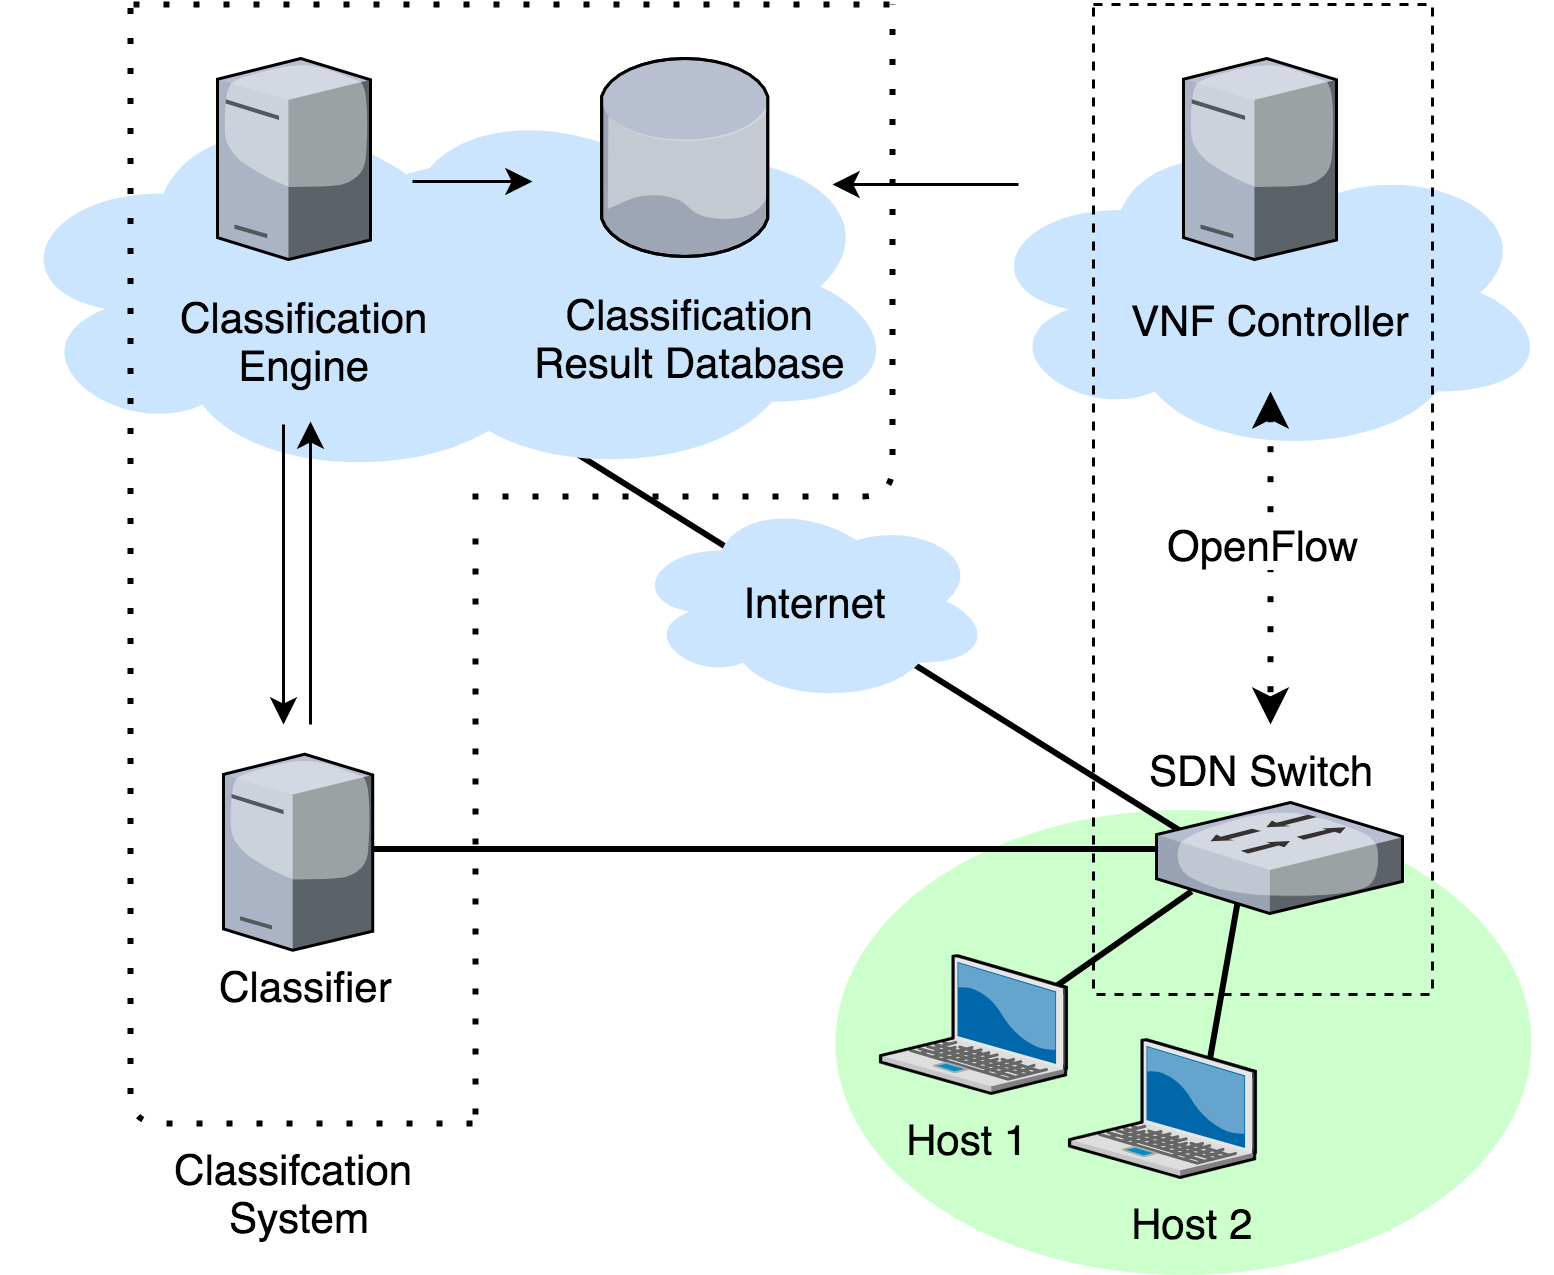
\includegraphics[width=3in]{./figures/classification_classifying}
\caption{Architecture of our application identification system in classifying phase}
\label{fig:classifcation_classifying}
\end{figure}

\subsection{Overall procedure of application identification}
In training phase, we generate some data needed by ML and the method based on inspecting DNS responses. In classifying phase, if a flow meet some requirement, we use the method based on inspecting DNS response to classify; otherwise, we use ML to classify.

\subsection{Procedure of Supervised ML in our system}
In training phase, the architecture is show in Fig I. Flow classification engine is to build classification model by training data from Trainer, and update the model when new training data comes. Trainer is to analyze traffic from mirror port to get flow attributes. After Trainer finishes calculating flow attributes of a flow, it gets ground truth of the flow from Scanner or App Meta Server to generate training data, and sends training data to flow classification engine. App Meta Server is to store mappings of 5-tuple and ground truth from Scanner, and accept queries from Trainer. Scanner is to get mappings of 5-tuple and ground truth from OS.
In classifying phase, the architecture is shown in Fig. Flow classification engine is to use flow attributes from Classifier and classification model to get a classification result, and sends classification result to Classifier. Classifier is to analyze traffic from mirror port to get flow attributes. After Classifier finishes calculating flow attributes of a flow, it use flow attributes to ask flow classification engine for classification result if needed.

\subsection{Flow attributes we adopted in ML}
In ML, when system calculates flow attributes, we only use transport layer information of packets which have payload. We use Application Round (APPR) proposed by [] to analyze flow behavior. We use number of packets, packet sizes, transmission time, transmission direction, throughput, and APPR to define flow attributes. There are 69 attributes in total, as defined in our previous work [].

\subsection{Algorithms we adopted in ML}
We use algorithms implemented by Weka, a famous open source ML tool developed at the University of Waikato. We call Weka Java API to build classification model. We use three algorithms, namely RandomSupSpace with RandomTree [], FilterClassifier with discretization and RandomTree [], and RandomCommittee with RandomTree [].

\subsection{Procedure of a method based on inspecting DNS response in our system}
In training phase, we collect the mappings of server IP and application name. A mapping of server IP and application name means the application has ever establish connection with the server whose IP is the server IP, and the server IP has ever occurred in any DNS response we have captured.
In classifying phase, we only use those mappings which have been used by one application to classify. When system detect a flow, we check whether source IP or destination IP of the flow match any server IP of those mappings. If it matches any server IP, we regard corresponding application name as classification result; otherwise, we use flow attributes of the flow and classification model to classify.



\section{Performance Evaluation}
\subsection{Multiple Table Performance}

\subsection{Accuracy of Application Identification }

\subsubsection{Testing data set}
Testing data set are mappings of flow attributes and ground truth (also called rules). This testing data set were generated by our system in our lab in National Tsing Hua University in Taiwan in 2016. We manually operated applications to generate traffic. After the system generated rules, it exported them into a file, because we wanted to do 10-fold cross validation on the testing data set. There are 14659 rules in total, and there are 137 applications if we view each platform version of an application as one application.
(提fig 1)

\subsubsection{Validation method}
Although the system can do online training and classifying, we do offline training and classifying. More specifically, when we did online training to analyze traffic, get ground truth, and export the rules into a file. We do 10-fold cross validation on the rules. There are 10 rounds in 10-fold cross validation. Each round, we split testing data set into training dataset and classifying dataset.

\subsubsection{Mapping of category names}
We do name mapping on training dataset before we use training data set to build classification model, and do name mapping on classifying data set before we use classifying data set to calculate accuracy. The main reason is that some application have different ground truth in different operating system.

\subsubsection{Accuracy matrices}
To evaluate accuracy, we used precision, recall and F-measure (also called F1 score), as shown in Eq. (1), Eq. (2), and Eq. (3) []. In each round in 10-fold cross validation, we calculate precision and recall of each category to calculate F1 score of each category. After ten rounds, we calculate average

%%




\newpage

\bibliographystyle{ieeetr}
\bibliography{paper}

\end{document}
